\chapter{Lattices: Even, Unimodular, \texorpdfstring{$E_8$}{E8} and \texorpdfstring{$U$}{U}}
\label{ch:lattices}

Every charge that has appeared in this book so far has been an integer: a momentum number
$n$, a winding number $w$, a vector $Z\in\Z^{2d}$ of both. Integers that can be added form a
\emph{lattice}, and the physics equips that lattice with an integer-valued inner product: for
the circle, the level-matching pairing $2nw$ of \cref{ch:circle}; for the torus, the form
$\eta$ of \cref{ch:narain,ch:odd}. In Part~IV the same structure returns in geometry. The
second cohomology of a K3 surface is a lattice of rank $22$ whose inner product counts
intersections of surfaces, and almost everything we shall say about K3 surfaces (their
moduli, their symmetries, the strings that propagate on them) is phrased in terms of that
lattice. The question of this chapter is therefore a purely algebraic one: \emph{what is an
integral lattice, which invariants distinguish one lattice from another, and what are the two
building blocks, $U$ and $E_8$, from which the K3 lattice is assembled?}

A student should care for two reasons. First, the classification is surprisingly rigid: an
indefinite lattice that is even and unimodular is determined by two integers, its signature.
This is why one can write down $H^2(K3,\Z)$ without ever seeing a K3 surface
(\cref{ch:k3lattice}). Secondly, the chapter is a good place to learn how finite, explicit
mathematics is handed to a proof assistant. Every statement about $E_8$ below is a statement
about one $8\times8$ integer matrix, and the Lean proofs are \emph{certificates}: an inverse
matrix, a triangular factorization, a sum of squares, each of which the kernel checks by
arithmetic.

Conventions. A lattice is written $\Lambda$, its pairing $(x\cdot y)$, and $x^2:=(x\cdot x)$.
Signatures are written $(n_+,n_-)$. For a lattice $\Lambda$ and an integer $m$, $\Lambda(m)$
is the same group with the pairing multiplied by $m$. Direct sums are orthogonal. These are
the conventions of our main source \source{Huy §14.0.1--0.2, ll.~12645--12705}.

%=====================================================================================
\section{Integral lattices and Gram matrices}\label{sec:lattices:gram}

\begin{definition}[Lattice]\label{def:lattices:lattice}
A \emph{lattice}\index{lattice} is a free $\Z$-module $\Lambda$ of finite rank $n$ together
with a symmetric bilinear form $(\;\cdot\;)\colon\Lambda\times\Lambda\to\Z$ which is
non-degenerate: if $(x\cdot y)=0$ for all $y$, then $x=0$.
\source{Huy §14.0.1, ll.~12645--12649}
\end{definition}

``Free of rank $n$'' means that there is a basis $e_1,\dots,e_n$ such that every element is
uniquely $x=\sum_i x_ie_i$ with $x_i\in\Z$. Once a basis is chosen, the pairing is encoded in
the \emph{Gram matrix}\index{Gram matrix}
\begin{equation}\label{eq:lattices:gram}
 G_{ij}:=(e_i\cdot e_j),\qquad (x\cdot y)=\sum_{i,j}x_iG_{ij}y_j=x^{\mathsf T}Gy ,
\end{equation}
a symmetric integer matrix; non-degeneracy is the statement $\det G\neq0$. Note what is
\emph{not} assumed: the form need not be positive. The word ``lattice'' may suggest a grid of
points in Euclidean space, but the lattices of string theory are mostly \emph{indefinite}:
they contain nonzero vectors with $x^2=0$ and vectors with $x^2<0$.

\paragraph{Change of basis.} A second basis $e'_j=\sum_iP_{ij}e_i$ is related to the first by
an integer matrix $P$ whose inverse is also an integer matrix, that is $P\in GL(n,\Z)$, and
then $\det P=\pm1$ (because $\det P\cdot\det P^{-1}=1$ in $\Z$). The Gram matrix changes by a
\emph{congruence},
\begin{equation}\label{eq:lattices:congruence}
 G'=P^{\mathsf T}GP,\qquad P\in GL(n,\Z).
\end{equation}
A lattice is thus an equivalence class of symmetric integer matrices under
\eqref{eq:lattices:congruence}, and an \emph{invariant} of the lattice is any quantity that
does not change under it. Two lattices are \emph{isomorphic}, $\Lambda\cong\Lambda'$, if there
is a group isomorphism preserving the pairing; an isomorphism of $\Lambda$ with itself is an
\emph{isometry}, and the isometries form the \emph{orthogonal group}\index{orthogonal group
of a lattice}
\begin{equation}\label{eq:lattices:OLambda}
 O(\Lambda)=\{\,g\in GL(n,\Z)\;:\;g^{\mathsf T}Gg=G\,\}.
\end{equation}
For $G=\eta$ this is the T-duality group $\Odd{d}$ of \cref{ch:odd}. Deciding whether two
given Gram matrices are congruent is hard in general, which is why invariants matter.

\begin{definition}[Even and odd]\label{def:lattices:even}
A lattice is \emph{even}\index{even lattice} if $x^2\in2\Z$ for every $x\in\Lambda$, and
\emph{odd}\index{odd lattice} otherwise. \source{Huy §14.0.1, ll.~12649--12651}
\end{definition}

Evenness is a condition on infinitely many vectors, but it can be read off from $n$ numbers.

\begin{lemma}[Evenness from the diagonal]\label{lem:lattices:evendiag}
Let $G$ be a symmetric integer matrix. Then $x^{\mathsf T}Gx$ is even for every $x\in\Z^n$ if
and only if every diagonal entry $G_{ii}$ is even.
\end{lemma}
\begin{proof}
Separate the diagonal terms from the off-diagonal ones and use $G_{ij}=G_{ji}$:
\begin{equation}\label{eq:lattices:evensplit}
 x^{\mathsf T}Gx=\sum_iG_{ii}x_i^2+\sum_{i\neq j}G_{ij}x_ix_j
 =\sum_iG_{ii}x_i^2+2\sum_{i<j}G_{ij}x_ix_j .
\end{equation}
The second sum is even whatever the $G_{ij}$ are. If all $G_{ii}$ are even, the first sum is
even too. Conversely, $x=e_i$ gives $x^{\mathsf T}Gx=G_{ii}$.
\end{proof}

The ``if'' direction is the Lean theorem \lean{even\_quadratic\_form\_of\_even\_diag} of
\cref{sec:lattices:lean}; its proof is exactly the splitting \eqref{eq:lattices:evensplit},
with the matrix written as diagonal plus strictly upper triangular plus the transpose of the
latter. Symmetry is essential: for the non-symmetric matrix
$\bigl(\begin{smallmatrix}0&1\\0&0\end{smallmatrix}\bigr)$ the diagonal is even but
$x^{\mathsf T}Gx=x_1x_2$ is odd at $x=(1,1)$.

\begin{example}[Three lattices of rank at most two]\label{ex:lattices:small}
(i) $\langle m\rangle$ denotes the rank-one lattice $\Z e$ with $e^2=m$. It is even exactly
when $m$ is even. (ii) $\langle1\rangle\oplus\langle-1\rangle$ has
$G=\diag(1,-1)$ and $x^2=x_1^2-x_2^2$; it is odd. (iii) The lattice with
$G=\bigl(\begin{smallmatrix}0&1\\1&0\end{smallmatrix}\bigr)$ has $x^2=2x_1x_2$ and is even.
Lattices (ii) and (iii) have the same rank and, as we shall see, the same determinant and the
same signature. They are nevertheless not isomorphic, because one is even and the other is
not, and parity is an invariant.
\end{example}

\begin{physicsbox}[Why string theory wants even lattices]
For a closed string on a circle the level-matching condition of \cref{ch:circle} reads
$N-\tilde N=nw$. The right-hand side is one half of the norm of the charge vector
$(n,w)$ in the lattice (iii) above. Level matching can be satisfied by integer oscillator
levels only if that half-norm is an integer, that is, if the lattice is even. For $d$ compact
directions the statement is that the momenta $(p_L,p_R)$ form an even lattice with
$p_L^2-p_R^2=2m_in^i\in2\Z$, and that this lattice is self-dual
(\cref{sec:lattices:dual}) \source{GPR §2.4, ll.~1249--1255}. The two conditions together
are what modular invariance of the worldsheet theory on a torus requires
\source{Asp §3.5, ll.~1987--1988}. The usual refinement is that evenness gives invariance
of the partition function under $\tau\to\tau+1$ and self-duality gives invariance under
$\tau\to-1/\tau$, by Poisson resummation over the lattice; this is standard, is not spelled
out in the sources of this book's library, and is the subject of \cref{ch:narain}.
\end{physicsbox}

%=====================================================================================
\section{The dual lattice, the discriminant and unimodularity}\label{sec:lattices:dual}

\subsection{The discriminant}
Under the congruence \eqref{eq:lattices:congruence},
$\det G'=(\det P)^2\det G=\det G$. The determinant of a Gram matrix is therefore an invariant
of the lattice, the \emph{discriminant}\index{discriminant}
$\operatorname{disc}\Lambda:=\det G$ \source{Huy §14.0.1, ll.~12651--12652}. Its sign and its
absolute value both carry information, and both have a concrete meaning which we now derive.

\subsection{The dual lattice}
Extend the pairing $\Q$-linearly to $\Lambda_\Q:=\Lambda\otimes\Q$, the rational vector
space with the same basis. The \emph{dual lattice}\index{dual lattice} is
\begin{equation}\label{eq:lattices:dualdef}
 \Lambda^*:=\{\,x\in\Lambda_\Q\;:\;(x\cdot y)\in\Z\ \text{for all }y\in\Lambda\,\},
\end{equation}
which is a concrete model of $\operatorname{Hom}_\Z(\Lambda,\Z)$
\source{Huy §14.0.1, ll.~12659--12666}. Because the pairing is integral on $\Lambda$, we have
$\Lambda\subseteq\Lambda^*$. The dual lattice has the \emph{dual basis} $e_1^*,\dots,e_n^*$
defined by $(e_i^*\cdot e_j)=\delta_{ij}$. To find it, write
$e_i^*=\sum_kC_{ik}e_k$ with rational $C$; the defining condition is
$\sum_kC_{ik}G_{kj}=\delta_{ij}$, so
\begin{equation}\label{eq:lattices:dualbasis}
 e_i^*=\sum_k(G^{-1})_{ik}\,e_k,\qquad (e_i^*\cdot e_j^*)=(G^{-1}GG^{-1})_{ij}=(G^{-1})_{ij}.
\end{equation}
In words: \emph{the Gram matrix of the dual lattice is the inverse Gram matrix}. In the other
direction, $e_j=\sum_iG_{ji}e_i^*$, since both sides have the same pairings with all $e_k$.
In coordinates with respect to the dual basis, $\Lambda^*=\Z^n$ and $\Lambda=G\,\Z^n$.
The index of the subgroup $G\Z^n\subseteq\Z^n$ is $|\det G|$ (bring $G$ to diagonal form
$\diag(d_1,\dots,d_n)$ by integer row and column operations, which change neither the index
nor $|\det G|$; for a diagonal matrix the quotient is $\prod_i\Z/d_i\Z$). Hence:

\begin{proposition}\label{prop:lattices:index}
The \emph{discriminant group}\index{discriminant group} $A_\Lambda:=\Lambda^*/\Lambda$ is a
finite abelian group of order $|\operatorname{disc}\Lambda|$.
\source{Huy §14.0.1, ll.~12667--12672}
\end{proposition}

\begin{example}[The lattice $A_2$]\label{ex:lattices:A2}
Let $G=\bigl(\begin{smallmatrix}2&-1\\-1&2\end{smallmatrix}\bigr)$, the Gram matrix of two
vectors of length $\sqrt2$ at an angle of $120^\circ$ (the hexagonal lattice). Then
$\det G=3$ and $G^{-1}=\frac13\bigl(\begin{smallmatrix}2&1\\1&2\end{smallmatrix}\bigr)$. The
dual basis vector $e_1^*=\frac13(2e_1+e_2)$ is not in $\Lambda$, but $3e_1^*$ is, and
$e_2^*=2e_1^*-e_1$ differs from $2e_1^*$ by a lattice vector. So
$A_\Lambda\cong\Z/3\Z$, generated by the class of $e_1^*$, of order $3=\det G$ as
\cref{prop:lattices:index} demands. The norm $(e_1^*)^2=\frac23$ is well defined modulo $2$
on $A_\Lambda$; this is the \emph{discriminant form} $q_\Lambda\colon A_\Lambda\to\Q/2\Z$ of
an even lattice \source{Huy §14.0.1, ll.~12682--12690}, which will be needed for sublattices
of the K3 lattice in \cref{ch:k3lattice}.
\end{example}

\subsection{Unimodular lattices}
\begin{definition}\label{def:lattices:unimodular}
A lattice is \emph{unimodular}\index{unimodular lattice} (or
\emph{self-dual}\index{self-dual lattice}) if $\Lambda^*=\Lambda$; equivalently if $A_\Lambda$
is trivial; equivalently if $\operatorname{disc}\Lambda=\pm1$.
\source{Huy §14.0.1, ll.~12672--12673}
\end{definition}

The equivalences are \cref{prop:lattices:index}. A fourth equivalent form is the one that a
computer can check most cheaply.

\begin{lemma}[Inverse certificate]\label{lem:lattices:certificate}
A symmetric integer matrix $G$ satisfies $\det G=\pm1$ if and only if there is an
\emph{integer} matrix $H$ with $HG=\mathbf 1$.
\end{lemma}
\begin{proof}
If $HG=\mathbf 1$ with $H$ integral, then $\det H\cdot\det G=1$ is a factorization of $1$ in
$\Z$, so $\det G=\pm1$. Conversely, Cramer's rule gives $G^{-1}=\operatorname{adj}(G)/\det G$,
where the adjugate $\operatorname{adj}(G)$ is a matrix of minors of $G$ and hence integral; if
$\det G=\pm1$, then $H=\pm\operatorname{adj}(G)$ is integral.
\end{proof}

By \eqref{eq:lattices:dualbasis} the lemma says: $\Lambda$ is unimodular exactly when the dual
basis vectors already lie in $\Lambda$. The first half of the proof is the Lean lemma
\lean{isUnimodular\_of\_mul\_eq\_one}. It is the workhorse of the formalization, because it
replaces the computation of an $8\times8$ determinant (a sum of $8!=40320$ terms in the
Leibniz expansion) by the verification of $64$ integer identities.

\begin{pitfallbox}[Unimodular does not mean ``$\det=+1$'', and says nothing about the sign of
the form]
The three lattices $\langle1\rangle\oplus\langle1\rangle$,
$\langle1\rangle\oplus\langle-1\rangle$ and
$U=\bigl(\begin{smallmatrix}0&1\\1&0\end{smallmatrix}\bigr)$ are all unimodular, with
discriminants $+1,-1,-1$. The rank-$8$ lattices $E_8$ and $U^{\oplus4}$ are both even and
unimodular with discriminant $+1$, yet the first is positive definite and the second has
signature $(4,4)$. To distinguish them one needs the signature, which is the subject of the
next section; for $E_8$ it requires a separate proof (\cref{sec:lattices:posdef}).
\end{pitfallbox}

\subsection{Sums, twists and sublattices}
For an orthogonal direct sum the Gram matrix is block diagonal, so
$\operatorname{disc}(\Lambda_1\oplus\Lambda_2)=\operatorname{disc}\Lambda_1\cdot
\operatorname{disc}\Lambda_2$, and a sum of even (unimodular) lattices is even (unimodular).
For the twist, $\operatorname{disc}\Lambda(m)=m^{\rk\Lambda}\operatorname{disc}\Lambda$
\source{Huy §14.0.3, ll.~12819--12823}. If $\Lambda_1\subseteq\Lambda$ is a sublattice of
the same rank, a basis of $\Lambda_1$ is $e'=eP$ with an integer matrix $P$ of
$|\det P|=(\Lambda:\Lambda_1)$, the index. Then $G_1=P^{\mathsf T}GP$ gives
\begin{equation}\label{eq:lattices:indexformula}
 \operatorname{disc}\Lambda_1=\operatorname{disc}\Lambda\cdot(\Lambda:\Lambda_1)^2
 \qquad\text{\source{Huy eq.~(0.1), ll.~12708--12710}} .
\end{equation}
This formula is a quick way to prove unimodularity: if a lattice of discriminant $4$ has an
integral overlattice of index $2$, the overlattice is unimodular. We use it for $E_8$ in
\cref{ex:lattices:D8plus}.

%=====================================================================================
\section{Signature}\label{sec:lattices:signature}

Over the real numbers every non-degenerate symmetric bilinear form can be diagonalized with
entries $\pm1$: there is a real invertible $P$ with
$P^{\mathsf T}GP=\diag(1,\dots,1,-1,\dots,-1)$. The numbers $n_+$ and $n_-$ of positive and
negative entries form the \emph{signature}\index{signature of a lattice} $(n_+,n_-)$, and
$\tau:=n_+-n_-$ is the \emph{index}. A lattice is \emph{definite} if $n_+=0$ or $n_-=0$ and
\emph{indefinite}\index{indefinite lattice} otherwise \source{Huy §14.0.1, ll.~12653--12658}.
The definition makes sense because of

\begin{theorem}[Sylvester's law of inertia]\label{thm:lattices:sylvester}
\index{Sylvester's law of inertia}
The numbers $n_\pm$ do not depend on the diagonalizing matrix $P$.
\end{theorem}
\begin{proof}
Two diagonalizations give two splittings $\R^n=V_+\oplus V_-=V'_+\oplus V'_-$, where the
form is positive definite on $V_+,V'_+$ and negative definite on $V_-,V'_-$, and
$n_+=\dim V_+$, $n'_+=\dim V'_+$. A vector $x\in V_+\cap V'_-$ has $x^2>0$ unless $x=0$, and
also $x^2\le0$; so $V_+\cap V'_-=0$, hence $\dim V_++\dim V'_-\le n=\dim V'_++\dim V'_-$,
that is $n_+\le n'_+$. By symmetry $n_+=n'_+$.
\end{proof}

Two remarks make the signature computable. First, the sign of the discriminant is
$(-1)^{n_-}$, because $\det(P^{\mathsf T}GP)=(\det P)^2\det G$. Secondly, $P$ need not be
integral: \emph{any} real or rational congruence to a diagonal matrix reveals the signature,
and one reads off the signs of the diagonal entries. The standard way to produce such a
congruence is Gaussian elimination without row exchanges, which factorizes
\begin{equation}\label{eq:lattices:LDL}
 G=LDL^{\mathsf T},\qquad L\ \text{unit lower triangular},\quad D=\diag(d_1,\dots,d_n),
\end{equation}
whenever no zero pivot is met. Then $x^{\mathsf T}Gx=\sum_kd_ky_k^2$ with $y=L^{\mathsf T}x$,
which is ``completing the square'' one variable at a time. Since the upper-left $k\times k$
block of \eqref{eq:lattices:LDL} is the same factorization of the upper-left block $G_{(k)}$
of $G$, and $\det L_{(k)}=1$, the pivots are ratios of leading principal minors:
\begin{equation}\label{eq:lattices:pivots}
 d_1d_2\cdots d_k=\det G_{(k)},\qquad d_k=\frac{\det G_{(k)}}{\det G_{(k-1)}} .
\end{equation}
In particular $G$ is positive definite if and only if all pivots are positive, if and only
if all leading principal minors are positive (Sylvester's criterion).

Signatures add under direct sums, and the twist by $-1$ exchanges $n_+$ and $n_-$.
In physics language, $n_+$ and $n_-$ count left- and right-moving compact bosons
(\cref{ch:narain}); in geometry, for the lattice $H^2(X,\Z)$ of a four-manifold, they count
self-dual and anti-self-dual harmonic two-forms (\cref{ch:k3}).

%=====================================================================================
\section{The hyperbolic plane \texorpdfstring{$U$}{U}}\label{sec:lattices:U}

\begin{definition}\label{def:lattices:U}
The \emph{hyperbolic plane}\index{hyperbolic plane $U$} is the lattice $U=\Z e\oplus\Z f$
with $e^2=f^2=0$ and $(e\cdot f)=1$, that is, with Gram matrix
$\bigl(\begin{smallmatrix}0&1\\1&0\end{smallmatrix}\bigr)$.
\source{Huy §14.0.3, ll.~12781--12787}
\end{definition}

For $x=ae+bf$ we have $x^2=2ab$. The lattice is even (the diagonal of $G$ is zero;
\cref{lem:lattices:evendiag}), and unimodular with $\operatorname{disc}U=-1$; indeed $G^2=
\mathbf1$, so $G$ is its own integer inverse, and the dual basis is $e^*=f$, $f^*=e$. The
change of variables $u=e+f$, $v=e-f$ gives $u^2=2$, $v^2=-2$, $(u\cdot v)=0$, or in matrix form
\begin{equation}\label{eq:lattices:Ucongruence}
 P^{\mathsf T}\begin{pmatrix}0&1\\1&0\end{pmatrix}P=\begin{pmatrix}2&0\\0&-2\end{pmatrix},
 \qquad P=\begin{pmatrix}1&1\\1&-1\end{pmatrix},
\end{equation}
so by \cref{thm:lattices:sylvester} the signature is $(1,1)$. Note that $\det P=-2$: the
vectors $u,v$ span a sublattice $\langle2\rangle\oplus\langle-2\rangle$ of index $2$ and
discriminant $-4=(-1)\cdot2^2$, in agreement with \eqref{eq:lattices:indexformula}. Over
$\Z$ the lattice $U$ \emph{cannot} be diagonalized, since a diagonal unimodular lattice of
rank two is odd (\cref{ex:lattices:small}). Finally $U(-1)\cong U$, by $e\mapsto e$,
$f\mapsto-f$ \source{Huy §14.0.3, l.~12831}.

\begin{figure}[t]
\centering
\begin{tikzpicture}[scale=1.12,>=Stealth]
 \draw[gray!35,very thin] (-2.6,-2.6) grid (2.6,2.6);
 \foreach \a in {-2,...,2}\foreach \b in {-2,...,2}\fill[black!60] (\a,\b) circle (1.2pt);
 \draw[->,thick] (-2.8,0)--(3.0,0) node[right,font=\small]{$a$ (along $e$)};
 \draw[->,thick] (0,-2.8)--(0,3.0) node[above,font=\small]{$b$ (along $f$)};
 \draw[blue!70!black,domain=0.385:2.6,smooth,samples=40] plot(\x,{1/\x});
 \draw[blue!70!black,domain=-2.6:-0.385,smooth,samples=40] plot(\x,{1/\x});
 \draw[red!70!black,domain=0.385:2.6,smooth,samples=40] plot(\x,{-1/\x});
 \draw[red!70!black,domain=-2.6:-0.385,smooth,samples=40] plot(\x,{-1/\x});
 \draw[dashed] (-2.5,-2.5)--(2.5,2.5);
 \node[font=\small,anchor=west] at (2.55,2.55) {mirror of $s_{e-f}$};
 \draw[->,very thick,blue!70!black] (0,0)--(1,1);
 \node[blue!70!black,font=\small,anchor=west,fill=white,inner sep=1pt] at (1.3,1.08) {$e+f$};
 \draw[->,very thick,red!70!black] (0,0)--(1,-1);
 \node[red!70!black,font=\small,anchor=west,fill=white,inner sep=1pt] at (1.3,-1.08) {$e-f$};
 \draw[->,very thick] (0,0)--(1,0);
 \node[font=\small,anchor=south west] at (1.0,0.0) {$e$};
 \draw[->,very thick] (0,0)--(0,1);
 \node[font=\small,anchor=east] at (-0.05,1.0) {$f$};
 \node[blue!70!black,font=\small,anchor=west] at (0.5,2.35) {$x^2=2$};
 \node[red!70!black,font=\small,anchor=west] at (0.5,-2.35) {$x^2=-2$};
\end{tikzpicture}
\caption{The hyperbolic plane $U$ in the coordinates $x=ae+bf$, where $x^2=2ab$. The two
axes are the isotropic (null) directions. The hyperbolas $x^2=\pm2$ each contain exactly two
lattice points, $\pm(e+f)$ and $\pm(e-f)$. The reflection $s_{e-f}$ of
\cref{sec:lattices:reflections} is the mirror image in the dashed line: it exchanges $e$ and
$f$.}\label{fig:lattices:U}
\end{figure}

\paragraph{Isometries.} A vector is \emph{isotropic} if its norm is zero and
\emph{primitive}\index{primitive vector} if it is not an integer multiple $kx'$, $|k|\ge2$,
of another lattice vector. An isometry $g$ of $U$ must send $e$ to a primitive isotropic
vector, and $2ab=0$ with $ae+bf$ primitive leaves only $\pm e,\pm f$. The image of $f$ is then
fixed by $g(f)^2=0$ and $(g(e)\cdot g(f))=1$. Hence
\begin{equation}\label{eq:lattices:OU}
 O(U)=\{\pm\mathbf1,\ \pm\bigl(\begin{smallmatrix}0&1\\1&0\end{smallmatrix}\bigr)\}
 \cong(\Z/2\Z)^2 \qquad\text{\source{Huy Ex.~14.2.1, ll.~13159--13164}} ,
\end{equation}
which is the group $O(1,1;\Z)$ found in \cref{ch:odd}. So $U$ is an indefinite lattice with a
\emph{finite} orthogonal group. This is exceptional and is tied to the existence of
isotropic vectors in rank two \source{Huy §14.2, ll.~13147--13157}; for $U^{\oplus d}$ with
$d\ge2$ the group $\Odd{d}$ is infinite.

\begin{physicsbox}[$U$ is the charge lattice of a circle]
Identify $a$ with the momentum number $n$ and $b$ with the winding number $w$ of a closed
string on a circle (\cref{ch:circle}). Then $\frac12x^2=nw$ is the right-hand side of the
level-matching condition, the two null directions are the pure-momentum and pure-winding
states, and the nontrivial isometry $e\leftrightarrow f$ is T-duality, $n\leftrightarrow w$
(\cref{ch:tduality}). The radius $R$ does not appear: the lattice $U$ with its pairing is the
same for all radii. What depends on $R$ is how $U\otimes\R=\R^{1,1}$ is split into a positive
line (left-movers) and a negative line (right-movers), and the mass formula measures the
position of a charge vector relative to that splitting. The moduli space of the circle is the
space of such splittings modulo $O(U)$. This picture generalizes verbatim to tori
($U^{\oplus d}$, \cref{ch:narain}) and to K3 surfaces (\cref{ch:stringsk3}). In Lean, the
Gram matrix \lean{hyperbolicU} is proved equal to the Narain Gram matrix of the older
library by \lean{hyperbolicU\_eq\_narain\_gram}; the identification of either matrix with a
physical string is a modelling statement and is not Tier~A.
\end{physicsbox}

\paragraph{$U$ always splits off.} If a lattice $\Lambda$ contains two vectors $e,f$ with
$e^2=f^2=0$ and $(e\cdot f)=1$, then $\Lambda=U\oplus U^\perp$. Indeed, for $\alpha\in\Lambda$
put $\alpha':=\alpha-(e\cdot\alpha)f-(f\cdot\alpha)e$. Then
$(\alpha'\cdot e)=(\alpha\cdot e)-(e\cdot\alpha)\cdot1-0=0$ and likewise
$(\alpha'\cdot f)=0$, so $\alpha'\in U^\perp$, and $\alpha$ is the sum of an element of $U$
and one of $U^\perp$ \source{Huy Ex.~14.0.3, ll.~12789--12794}. The argument uses only that
the Gram matrix of $e,f$ is invertible over $\Z$; it works for any unimodular sublattice. For
a non-unimodular sublattice $\Lambda_1$ it fails, and $\Lambda_1\oplus\Lambda_1^\perp$ is in
general only of finite index in $\Lambda$ \source{Huy eq.~(0.2), ll.~12717--12729}.

%=====================================================================================
\section{The classification of indefinite even unimodular lattices}
\label{sec:lattices:classification}

We have met three invariants of an even unimodular lattice: the rank, the discriminant
$\pm1$ and the signature. The discriminant is $(-1)^{n_-}$ and the rank is $n_++n_-$, so only
the signature is independent. The remarkable fact is that for indefinite lattices there is
nothing else.

\begin{theorem}[Classification; Tier~L]\label{thm:lattices:classification}
\index{classification of even unimodular lattices}
Let $(n_+,n_-)$ be given. An even unimodular lattice of signature $(n_+,n_-)$ exists if and
only if
\begin{equation}\label{eq:lattices:mod8}
 n_+-n_-\equiv0\pmod 8 .
\end{equation}
If $n_+>0$ and $n_->0$, the lattice is unique up to isomorphism; for $\tau=n_+-n_-\ge0$ it is
\begin{equation}\label{eq:lattices:II}
 II_{n_+,n_-}\;\cong\;E_8^{\oplus\tau/8}\oplus U^{\oplus n_-},
 \qquad\text{and for }\tau\le0:\quad
 II_{n_+,n_-}\cong E_8(-1)^{\oplus|\tau|/8}\oplus U^{\oplus n_+} .
\end{equation}
\TL\ \source{Huy Thm.~14.1.1 and Cor.~14.1.3, ll.~12906--12932; Asp §2.3, ll.~559--565}
\end{theorem}

Huybrechts calls the theorem a classical result of Milnor and refers for the proof to Milnor--Husemoller, \emph{Symmetric bilinear forms}, Ch.~II, and
Serre, \emph{A course in arithmetic}, Ch.~V
\source{Huy ll.~12906--12907; bibliography ll.~19517, 19808}.
Neither is in this book's library and the theorem is not formalized in the Lean development; everywhere in this
book it is Tier~L. We use it as a black box and we now unpack what it says.

\paragraph{Existence.} The ``if'' part is constructive once $E_8$ and $U$ are known to be
even and unimodular of signatures $(8,0)$ and $(1,1)$: the right-hand sides of
\eqref{eq:lattices:II} are even, unimodular, and have signature
$(8\cdot\tau/8+n_-,\,n_-)=(n_+,n_-)$. This part \emph{is} within reach of the elementary
methods of this chapter, and \cref{sec:lattices:E8,sec:lattices:posdef} supply it. The
``only if'' part, the congruence \eqref{eq:lattices:mod8}, is deep; we do not prove it. It is
the algebraic counterpart of the fact that a modular-invariant lattice partition function
needs $n_L-n_R\in8\Z$ \source{Asp §3.5, ll.~1987--1988}.

\paragraph{Uniqueness.} This is the part that is used most. Here are the instances that occur
in this book.
\begin{center}\small
\begin{tabular}{@{}llll@{}}\toprule
signature & $\tau$ & lattice & where it appears\\\midrule
$(1,1)$ & $0$ & $U$ & charge lattice of a circle (\cref{ch:circle})\\
$(d,d)$ & $0$ & $U^{\oplus d}$ & Narain lattice of $T^d$ (\cref{ch:narain})\\
$(1,9)$ & $-8$ & $E_8(-1)\oplus U$ & Enriques lattice \source{Huy ll.~12886--12893}\\
$(3,19)$ & $-16$ & $E_8(-1)^{\oplus2}\oplus U^{\oplus3}$ & $H^2(K3,\Z)$
 (\cref{ch:k3lattice})\\
$(4,20)$ & $-16$ & $E_8(-1)^{\oplus2}\oplus U^{\oplus4}$ & Mukai lattice $H^*(K3,\Z)$
 (\cref{ch:mukai})\\
$(1,25)$ & $-24$ & $E_8(-1)^{\oplus3}\oplus U$ & Niemeier lattices (\cref{ch:m24})\\
\bottomrule
\end{tabular}
\end{center}
The K3 row shows how the theorem is used in practice. Topology gives three facts about
$H^2(X,\Z)$ of a K3 surface $X$: it is unimodular (Poincar\'e duality), even (the manifold
is spin), and of signature $(3,19)$ (the signature theorem). The theorem then hands us the
Gram matrix without any further geometry
\source{Asp §2.3, ll.~523--636; Huy Prop.~1.3.5, ll.~600--609}. This argument is carried out
in \cref{ch:k3,ch:k3lattice}.

\begin{pitfallbox}[Definite lattices are not classified by their signature]
The uniqueness statement needs $n_\pm>0$. For definite lattices it fails badly: in rank $24$
there are $24$ different even unimodular negative definite lattices, the Niemeier lattices,
of which $E_8(-1)^{\oplus3}$ is the simplest \source{Huy §14.4.1, ll.~13741--13760}. They all
become isomorphic after adding one copy of $U$: $N\oplus U\cong II_{1,25}$
\source{Huy Cor.~14.4.1, ll.~13744--13746}. Conversely, inside the single lattice
$II_{1,25}$ there are $24$ inequivalent ways of choosing a primitive null vector
\source{Huy ll.~13754--13757}. Adding a hyperbolic plane erases the distinction between
definite lattices of the same rank.
\end{pitfallbox}

%=====================================================================================
\section{The lattice \texorpdfstring{$E_8$}{E8}}\label{sec:lattices:E8}

\subsection{From a graph to a Gram matrix}
To any graph $\Gamma$ with simple edges one associates a lattice $\Lambda(\Gamma)$ with one
basis vector $\alpha_i$ per vertex and
\begin{equation}\label{eq:lattices:graphlattice}
 (\alpha_i\cdot\alpha_j)=\begin{cases}2&i=j,\\-1&i,j\ \text{joined by an edge},\\
 0&\text{otherwise}\end{cases}
 \qquad\text{\source{Huy §14.0.3\,v), ll.~12835--12838}} .
\end{equation}
Such a lattice is even by \cref{lem:lattices:evendiag}. The connected graphs for which it is
positive definite are exactly the Dynkin diagrams\index{Dynkin diagram} of type $A_n$, $D_n$,
$E_6$, $E_7$, $E_8$ \source{Huy ll.~12839--12841}; the basis vectors are then called
\emph{simple roots}\index{simple root} and the Gram matrix is the \emph{Cartan
matrix}\index{Cartan matrix} of the corresponding simply-laced Lie algebra. Among all of
them only $E_8$ is unimodular: the discriminant groups are $\Z/(n+1)$ for $A_n$, of order
$4$ for $D_n$, and $\Z/3$, $\Z/2$, $0$ for $E_6,E_7,E_8$ \source{Huy ll.~12868--12872}.

\begin{figure}[t]
\centering
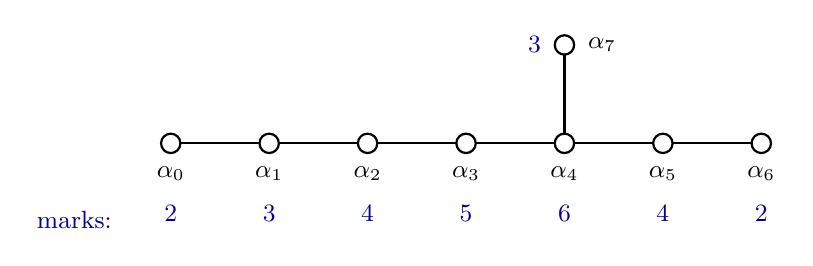
\begin{tikzpicture}[scale=1.25,
  nd/.style={circle,draw,thick,inner sep=0pt,minimum size=7pt,fill=white}]
 \draw[thick] (0,0)--(6,0);
 \draw[thick] (4,0)--(4,1);
 \foreach \i/\m in {0/2,1/3,2/4,3/5,4/6,5/4,6/2}{
   \node[nd] (n\i) at (\i,0) {};
   \node[below=5pt,font=\small] at (\i,0) {$\alpha_{\i}$};
   \node[below=19pt,font=\small,blue!60!black] at (\i,0) {$\m$};}
 \node[nd] (n7) at (4,1) {};
 \node[right=5pt,font=\small] at (4,1) {$\alpha_7$};
 \node[left=5pt,font=\small,blue!60!black] at (4,1) {$3$};
 \node[left,font=\small,blue!60!black] at (-0.5,-0.78) {marks:};
\end{tikzpicture}
\caption{The Dynkin diagram of $E_8$ in the labelling of the Lean file \lean{E8.lean}: a
chain $\alpha_0,\dots,\alpha_6$ with $\alpha_7$ attached to $\alpha_4$, so that the arms at
the branch node have $4$, $2$ and $1$ further nodes. The numbers in the second row are the
first row of the inverse Cartan matrix \eqref{eq:lattices:E8inv}; they are the coefficients
of the highest root.}\label{fig:lattices:dynkin}
\end{figure}

For the graph of \cref{fig:lattices:dynkin} the recipe \eqref{eq:lattices:graphlattice}
gives
\begin{equation}\label{eq:lattices:cartan}
 E_8:=\begin{pmatrix}
 2&-1&0&0&0&0&0&0\\ -1&2&-1&0&0&0&0&0\\ 0&-1&2&-1&0&0&0&0\\ 0&0&-1&2&-1&0&0&0\\
 0&0&0&-1&2&-1&0&-1\\ 0&0&0&0&-1&2&-1&0\\ 0&0&0&0&0&-1&2&0\\ 0&0&0&0&-1&0&0&2
 \end{pmatrix},
\end{equation}
which is the Lean matrix \lean{cartanE8}. The only entries off the tridiagonal band are the
two $-1$'s in positions $(4,7)$ and $(7,4)$, which record the extra edge.

\begin{pitfallbox}[Every book labels the nodes differently]
The matrix printed by Huybrechts \source{Huy §14.0.3\,iii), ll.~12796--12818} has its branch
at the third node of the chain and is not equal to \eqref{eq:lattices:cartan}; Bourbaki's
labelling is different again. The matrices are related by a permutation matrix $P$ as in
\eqref{eq:lattices:congruence}, so they define the same lattice. When comparing a formula
with Lean code, first match the labelling: the inverse matrix, the pivots and the highest
root all change their appearance under $P$.
\end{pitfallbox}

\subsection{The determinant from the diagram}\label{sec:lattices:det}
The determinant of a graph lattice can be computed by removing leaves.

\begin{lemma}[Leaf recursion]\label{lem:lattices:leaf}
Let $v$ be a vertex of $\Gamma$ joined to exactly one other vertex $u$. Then
\[
 \det\Lambda(\Gamma)=2\det\Lambda(\Gamma\setminus v)-\det\Lambda(\Gamma\setminus\{u,v\}) .
\]
\end{lemma}
\begin{proof}
Order the basis so that $u$ and $v$ come last. The Gram matrix is
\[
 G=\begin{pmatrix}G''&b&0\\ b^{\mathsf T}&2&-1\\0&-1&2\end{pmatrix},
\]
where $G''$ is the Gram matrix of $\Gamma\setminus\{u,v\}$. Expand along the last row. The
entry $2$ contributes $2\det\Lambda(\Gamma\setminus v)$. The entry $-1$ in position
$(n,n-1)$ contributes $(-1)\cdot(-1)^{2n-1}\det M=\det M$, where
$M=\bigl(\begin{smallmatrix}G''&0\\b^{\mathsf T}&-1\end{smallmatrix}\bigr)$ is obtained by
deleting the last row and the column of $u$; and $\det M=-\det G''$.
\end{proof}

For the chain $A_n$ the lemma gives $a_n=2a_{n-1}-a_{n-2}$ with $a_0=1$, $a_1=2$, hence
$\det A_n=n+1$. For $E_8$ take $v=\alpha_7$ and $u=\alpha_4$. Removing $\alpha_7$ leaves the
chain $A_7$; removing also $\alpha_4$ leaves $A_4\sqcup A_2$ (the nodes $0$--$3$ and $5$--$6$).
Therefore
\begin{equation}\label{eq:lattices:detE8}
 \det E_8=2\cdot8-5\cdot3=1 .
\end{equation}
The same computation for the diagram with a chain of $n-1$ nodes and the extra node attached
to the third node from one end gives $\det E_n=2n-3(n-3)=9-n$: the values $3,2,1$ for
$n=6,7,8$ match the orders of the discriminant groups quoted above, $\det E_9=0$ says that
the next diagram is degenerate, and $\det E_{10}=-1$ says that $E_{10}$ is again even and
unimodular, now indefinite (a numerical check finds signature $(9,1)$), hence isomorphic to
$E_8\oplus U$ by \cref{thm:lattices:classification}. The number $8$ is singled out as the
rank at which the determinant hits $1$. \Cref{eq:lattices:detE8} is a proof on the page; Lean obtains
$\det E_8=1$ by another route (\lean{cartanE8\_det}, below).

\subsection{The explicit inverse}
By \cref{lem:lattices:certificate}, $\det E_8=\pm1$ is equivalent to the existence of an
integer inverse. It is
\begin{equation}\label{eq:lattices:E8inv}
 E_8^{-1}=\begin{pmatrix}
 2&3&4&5&6&4&2&3\\3&6&8&10&12&8&4&6\\4&8&12&15&18&12&6&9\\5&10&15&20&24&16&8&12\\
 6&12&18&24&30&20&10&15\\4&8&12&16&20&14&7&10\\2&4&6&8&10&7&4&5\\3&6&9&12&15&10&5&8
 \end{pmatrix},
\end{equation}
the Lean matrix \lean{cartanE8Inv}. The reader should check a few entries of
$E_8^{-1}E_8=\mathbf1$ by hand. For the first row: the $(0,0)$ entry is
$2\cdot2+3\cdot(-1)=1$, the $(0,1)$ entry is $2\cdot(-1)+3\cdot2+4\cdot(-1)=0$, and the
$(0,4)$ entry, which feels the branch, is $-5+2\cdot6-4-3=0$. In general the first row
satisfies $2m_i=\sum_{j\sim i}m_j$ at every node except $\alpha_0$, where $2m_0-m_1=1$: each
mark is half the sum of its neighbours. This is a discrete harmonic condition, and it makes
the row easy to reconstruct from the diagram alone.

The inverse has a meaning. By \eqref{eq:lattices:dualbasis} its rows are the coordinates of
the dual basis vectors $\omega_i=\sum_j(E_8^{-1})_{ij}\alpha_j$ (the \emph{fundamental
weights}), with $(\omega_i\cdot\alpha_j)=\delta_{ij}$ and
$(\omega_i\cdot\omega_j)=(E_8^{-1})_{ij}$. For $A_2$ the fundamental weights were not in the
lattice (\cref{ex:lattices:A2}); for $E_8$ they are: \emph{the weight lattice of $E_8$
equals its root lattice}. The diagonal entries $2,6,12,20,30,14,4,8$ are the norms
$\omega_i^2$. Only $\omega_0$ has norm $2$, so it is itself a root,
$\omega_0=2\alpha_0+3\alpha_1+4\alpha_2+5\alpha_3+6\alpha_4+4\alpha_5+2\alpha_6+3\alpha_7$.
A computer enumeration (a symbolic check, not Tier~A) confirms that this is the highest of
the $120$ positive roots; its coefficients sum to $29$.

\subsection{Positive definiteness}\label{sec:lattices:posdef}
Evenness and $\det=1$ do not yet distinguish $E_8$ from $U^{\oplus4}$. We need the signature,
and we get it from the factorization \eqref{eq:lattices:LDL}. The leading principal minors of
\eqref{eq:lattices:cartan} are the determinants of $A_1,\dots,A_7$ and of $E_8$ itself, that
is $2,3,4,5,6,7,8,1$. By \eqref{eq:lattices:pivots} the pivots are
\begin{equation}\label{eq:lattices:pivotsE8}
 D=\diag\Bigl(2,\ \tfrac32,\ \tfrac43,\ \tfrac54,\ \tfrac65,\ \tfrac76,\ \tfrac87,\
 \tfrac18\Bigr),\qquad \prod_kd_k=1 .
\end{equation}
All are positive, so $E_8$ is positive definite, of signature $(8,0)$; the last pivot is
small but not zero (for the diagram $E_9$ of \cref{sec:lattices:det}, with one more node on
the long arm, the last pivot is $0/9=0$). To make
the argument checkable line by line, let us carry out the elimination. Write
$q(x):=x^{\mathsf T}E_8x=2\sum_ix_i^2-2\sum_{i\sim j}x_ix_j$, where the second sum runs over
the seven edges. Completing the square in $x_0$,
\[
 2x_0^2-2x_0x_1=2\bigl(x_0-\tfrac12x_1\bigr)^2-\tfrac12x_1^2 ,
\]
leaves $x_1$ with the coefficient $2-\frac12=\frac32$. Completing the square in $x_1$,
$\frac32x_1^2-2x_1x_2=\frac32(x_1-\frac23x_2)^2-\frac23x_2^2$, leaves $x_2$ with
$2-\frac23=\frac43$. Along the chain the pivot recursion is $d_{k+1}=2-1/d_k$, solved by
$d_k=(k+2)/(k+1)$. At the branch node $x_4$ is coupled to both $x_5$ and $x_7$, so the square
contains both, and a cross term $x_5x_7$ is generated which the next step removes. The result
is
\begin{equation}\label{eq:lattices:sos}
 q(x)=2y_0^2+\tfrac32y_1^2+\tfrac43y_2^2+\tfrac54y_3^2+\tfrac65y_4^2+\tfrac76y_5^2
 +\tfrac87y_6^2+\tfrac18y_7^2 ,
\end{equation}
\begin{equation}\label{eq:lattices:yvars}
\begin{aligned}
 y_0&=x_0-\tfrac12x_1, & y_1&=x_1-\tfrac23x_2, & y_2&=x_2-\tfrac34x_3, &
 y_3&=x_3-\tfrac45x_4,\\
 y_4&=x_4-\tfrac56x_5-\tfrac56x_7, & y_5&=x_5-\tfrac67x_6-\tfrac57x_7, &
 y_6&=x_6-\tfrac58x_7, & y_7&=x_7 .
\end{aligned}
\end{equation}
This is the identity $E_8=LDL^{\mathsf T}$ with $y=L^{\mathsf T}x$; the coefficients in
\eqref{eq:lattices:yvars} are the entries of the Lean matrix \lean{e8L}. Both the matrix
identity and the polynomial identity \eqref{eq:lattices:sos} were checked with sympy before
being given to Lean. Positive definiteness now follows in two steps. (a) $q(x)\ge0$, as a sum
of squares with positive weights. (b) If $q(x)=0$, then every $y_k=0$; reading
\eqref{eq:lattices:yvars} from the end, $x_7=0$, then $x_6=0$, $x_5=0$, \dots, $x_0=0$. The
substitution $x\mapsto y$ is invertible precisely because it is unit triangular.

\begin{example}[The sum of the simple roots]\label{ex:lattices:allones}
Take $x=(1,1,1,1,1,1,1,1)$, that is $\beta=\alpha_0+\dots+\alpha_7$. Directly,
$q=2\cdot8-2\cdot7=2$: eight vertices, seven edges. Through \eqref{eq:lattices:yvars},
\[
 y=\bigl(\tfrac12,\tfrac13,\tfrac14,\tfrac15,-\tfrac23,-\tfrac47,\tfrac38,1\bigr),\qquad
 q=\tfrac12+\tfrac16+\tfrac1{12}+\tfrac1{20}+\tfrac8{15}+\tfrac8{21}+\tfrac9{56}+\tfrac18=2 ,
\]
as one confirms with the common denominator $840$:
$420+140+70+42+448+320+135+105=1680$. So $\beta$ is a vector of norm $2$, a root. The same
count shows that for any tree the sum of all basis vectors has norm
$2(\#\text{vertices}-\#\text{edges})=2$.
\end{example}

\begin{example}[$E_8$ inside $\R^8$, and the $240$ roots]\label{ex:lattices:D8plus}
Positive definiteness means that $E_8$ can be drawn as a lattice of points in Euclidean
$\R^8$. A model which is standard (it is not taken from a source in this book's library; we
verify what we use) is
\[
 \Gamma_8:=\bigl\{x\in\Z^8\cup(\Z+\tfrac12)^8\;:\;\textstyle\sum_ix_i\in2\Z\bigr\}
\]
with the Euclidean inner product. In terms of the standard unit vectors
$\varepsilon_1,\dots,\varepsilon_8$ of $\R^8$ put
\[
 \alpha_k=\varepsilon_{7-k}-\varepsilon_{6-k}\ (0\le k\le5),\qquad
 \alpha_6=\tfrac12(\varepsilon_1+\varepsilon_8)-\tfrac12(\varepsilon_2+\dots+\varepsilon_7),
 \qquad\alpha_7=\varepsilon_1+\varepsilon_2 .
\]
These eight vectors lie in $\Gamma_8$ and their Gram matrix is exactly
\eqref{eq:lattices:cartan} (symbolic check; for instance
$(\alpha_5\cdot\alpha_6)=(\varepsilon_2-\varepsilon_1)\cdot\alpha_6=-\frac12-\frac12=-1$ and
$(\alpha_6\cdot\alpha_7)=\frac12-\frac12=0$). Unimodularity is visible without any
determinant: the integer vectors with even coordinate sum form the lattice $D_8$ of index $2$
in $\Z^8$, so $\operatorname{disc}D_8=1\cdot2^2=4$ by \eqref{eq:lattices:indexformula}, and
$\Gamma_8\supset D_8$ has index $2$, so $\operatorname{disc}\Gamma_8=4/2^2=1$. Since the
$\alpha_k$ span a sublattice of $\Gamma_8$ of discriminant $1$, the same formula shows that
the index is $1$: they span all of $\Gamma_8$.

The roots can now be counted. Integer vectors of norm $2$ are $\pm\varepsilon_i\pm
\varepsilon_j$ with $i<j$: $4\binom82=112$ of them, all of even sum. Half-integer vectors of
norm $2$ have all coordinates $\pm\frac12$ with an even number of minus signs: $2^7=128$.
Together $112+128=240$ roots\index{roots of $E_8$}, in agreement with
\source{Huy Ex.~14.2.3, ll.~13197--13201}. A computer search that starts from the simple
roots of \eqref{eq:lattices:cartan} and closes under reflections also stops at $240$ vectors
(symbolic check).
\end{example}

\subsection{\texorpdfstring{$E_8(-1)$}{E8(-1)}}
In geometry the form is negative on the relevant classes: the exceptional curves
$C_i\cong\mathbb P^1$ of the minimal resolution of an $E_8$ surface singularity
$x^2+y^3+z^5=0$ have $C_i^2=-2$ and meet each other according to the $E_8$ Dynkin diagram
\source{Huy §14.0.3\,v), ll.~12842--12860}. The lattice that occurs in $H^2(K3,\Z)$ is
therefore the twist $E_8(-1)$ with Gram matrix $-E_8$, which is even, unimodular (its
discriminant is $(-1)^8\cdot1=1$) and negative definite \source{Huy ll.~12829--12831}. In
Lean it is \lean{e8Neg}. The Lie algebra $E_8$ and the gauge group of the heterotic string
play no role in this chapter; only the lattice does.

%=====================================================================================
\section{Reflections and the Weyl group}\label{sec:lattices:reflections}

\subsection{Reflections in \texorpdfstring{$(-2)$}{(-2)}-vectors}
In a real vector space with a non-degenerate symmetric form, the reflection in the
hyperplane orthogonal to a vector
$\delta$ with $\delta^2\ne0$ is
\begin{equation}\label{eq:lattices:reflgeneral}
 s_\delta(x)=x-2\,\frac{(x\cdot\delta)}{\delta^2}\,\delta
 \qquad\text{\source{Huy §7.5.4, ll.~6031--6034}} .
\end{equation}
It fixes $\delta^\perp$ and sends $\delta\mapsto-\delta$. On a lattice this map is in general
not defined over $\Z$, because of the denominator $\delta^2$. It \emph{is} integral when
$\delta^2=\pm1$ or $\pm2$. In an even lattice the first case cannot occur, and we are left
with $\delta^2=\pm2$. A vector with $\delta^2=-2$ is called a \emph{root}\index{root} or
\emph{$(-2)$-class}, and for it \eqref{eq:lattices:reflgeneral} becomes
\begin{equation}\label{eq:lattices:refl}
 s_\delta(x)=x+(x\cdot\delta)\,\delta ,\qquad\text{as a matrix}\quad
 S_\delta=\mathbf1+\delta\delta^{\mathsf T}G
 \qquad\text{\source{Huy §14.2.1, ll.~13166--13176}} ,
\end{equation}
where $\delta$ is a column vector and we used $(x\cdot\delta)=\delta^{\mathsf T}Gx$. (For a
positive definite lattice such as $E_8$ one uses vectors of norm $+2$ and
$s_\delta(x)=x-(x\cdot\delta)\delta$; passing to $E_8(-1)$ changes both signs and gives the
same linear map.)

\begin{proposition}\label{prop:lattices:reflection}
Let $G$ be a symmetric integer matrix, $\delta\in\Z^n$, $N:=\delta^{\mathsf T}G\delta$ and
$S:=\mathbf1+\delta\delta^{\mathsf T}G$. Then
\begin{equation}\label{eq:lattices:reflidentity}
 S^{\mathsf T}GS-G=(2+N)\,G\delta\delta^{\mathsf T}G,\qquad
 S^2-\mathbf1=(2+N)\,\delta\delta^{\mathsf T}G .
\end{equation}
In particular, if $N=-2$ then $S$ is an isometry of $G$ and an involution.
\end{proposition}
\begin{proof}
The key is that $\delta^{\mathsf T}G\delta$ is a number, so
$(\delta\delta^{\mathsf T}G)(\delta\delta^{\mathsf T}G)=\delta(\delta^{\mathsf T}G\delta)
\delta^{\mathsf T}G=N\,\delta\delta^{\mathsf T}G$. Hence
$S^2=\mathbf1+2\delta\delta^{\mathsf T}G+N\delta\delta^{\mathsf T}G$. Similarly, with
$S^{\mathsf T}=\mathbf1+G\delta\delta^{\mathsf T}$ (here symmetry of $G$ is used),
\[
 S^{\mathsf T}GS=(\mathbf1+G\delta\delta^{\mathsf T})\,G\,(\mathbf1+\delta\delta^{\mathsf T}G)
 =G+2\,G\delta\delta^{\mathsf T}G+N\,G\delta\delta^{\mathsf T}G . \qedhere
\]
\end{proof}

The factor $(2+N)$ explains why the norm $-2$ is special for the formula
\eqref{eq:lattices:refl}. The Lean theorems \lean{reflection\_isometry} and
\lean{reflection\_involution} are the two consequences at $N=-2$, for arbitrary rank; the
general identities \eqref{eq:lattices:reflidentity} are proved above on the page and were
also checked with sympy, but are not themselves Lean theorems.

\begin{example}[T-duality is a reflection]\label{ex:lattices:Treflection}
In $U$ the vector $\delta=e-f$ has $\delta^2=-2$, and
$s_\delta(e)=e+(e\cdot(e-f))(e-f)=e-(e-f)=f$. So the reflection $s_{e-f}$ exchanges $e$ and
$f$ (\cref{fig:lattices:U}): with the identification of \cref{sec:lattices:U}, the T-duality
$n\leftrightarrow w$ of a circle is the reflection in the $(-2)$-vector $e-f$. The only roots
of $U$ are $\pm(e-f)$, since $2ab=-2$ forces $(a,b)=\pm(1,-1)$. Hence the Weyl group of $U$
is $\Z/2\Z$, a proper subgroup of $O(U)\cong(\Z/2\Z)^2$ \source{Huy ll.~13181--13182}; the
element $-\mathbf1$ is not a product of reflections in roots.
\end{example}

\begin{example}[A simple reflection of $E_8(-1)$]\label{ex:lattices:simplerefl}
Take $G=-E_8$ and $\delta=\alpha_4$, the branch node. Then $(x\cdot\alpha_4)=-(E_8x)_4
=x_3-2x_4+x_5+x_7$, so $s_{\alpha_4}$ changes only the fourth coordinate:
\[
 s_{\alpha_4}(x)=(x_0,x_1,x_2,x_3,\;x_3-x_4+x_5+x_7,\;x_5,x_6,x_7) .
\]
In particular $s_{\alpha_4}(\alpha_3)=\alpha_3+\alpha_4$, again a root, and
$s_{\alpha_4}(\alpha_4)=-\alpha_4$. Applying it twice returns $x_3-(x_3-x_4+x_5+x_7)+x_5+x_7
=x_4$, as it must.
\end{example}

\subsection{The Weyl group}
The \emph{Weyl group}\index{Weyl group} $W(\Lambda)\subseteq O(\Lambda)$ is the subgroup
generated by all reflections $s_\delta$ in roots \source{Huy §14.2.1, ll.~13177--13180}. The
following facts are Tier~L and are not formalized.
\begin{itemize}[leftmargin=*,itemsep=1pt]
\item For $E_8(-1)$, which has $240$ roots, the Weyl group has order
 $2^{14}\cdot3^5\cdot5^2\cdot7=4!\cdot6!\cdot8!=696\,729\,600$ and is the whole orthogonal
 group $O(E_8(-1))$ \source{Huy Ex.~14.2.3, ll.~13197--13201}. That it is generated by the
 eight \emph{simple} reflections $s_{\alpha_0},\dots,s_{\alpha_7}$ is standard Lie theory
 (not checked against a source in this book's library).
\item For the K3 lattice, every isometry of trivial spinor norm (equivalently, every
 isometry preserving the orientation of the three positive directions) is a product of
 reflections in $(-2)$-classes \source{Huy Thm.~14.2.2, ll.~13184--13195; §7.5.4,
 ll.~6028--6043}. This is the lattice-theoretic input to the global structure of the K3
 moduli space in \cref{ch:k3lattice,ch:stringsk3}.
\item In general $W$ can have infinite index in $O(\Lambda)$ \source{Huy ll.~13205--13210}.
\end{itemize}

\begin{physicsbox}[Reflections as monodromies]
Reflections in $(-2)$-classes are what a K3 surface does to its own cohomology when it is
taken around a singular point of its moduli space. If a family of K3 surfaces degenerates by
shrinking a sphere $C$ with $C^2=-2$ to a point (an $A_1$ singularity), then transporting
$H^2(X,\Z)$ once around the degeneration acts as the reflection $s_\delta$ in the class
$\delta=[C]$ \source{Huy §6, ll.~5398--5401}. This is the Picard--Lefschetz
formula\index{Picard--Lefschetz reflection}. In type~IIA string theory on a K3 surface, a
shrinking sphere means that a brane wrapped on it becomes massless, and a non-abelian gauge
symmetry appears whose roots are the $(-2)$-classes of the shrunken spheres; the roots all
have the same length, so the gauge algebra is of ADE type \TL\
\source{Asp §4.3, ll.~2464--2485, 2551--2565}; see \cref{ch:stringsk3}. The same source
notes that the simplest instance is the circle, where at a special radius a pair
$\pm\alpha$ of charge vectors enhances $U(1)$ to $SU(2)$ \source{Asp ll.~2472--2477}. Compare \cref{ex:lattices:Treflection}: for the circle the
reflection $s_{e-f}$ is T-duality, whose fixed point is the self-dual radius of
\cref{ch:tduality}.
\end{physicsbox}

%=====================================================================================
\section{What the machine has checked}\label{sec:lattices:lean}

The five files \lean{Basic.lean}, \lean{E8.lean}, \lean{E8PosDef.lean},
\lean{Hyperbolic.lean} and \lean{Reflection.lean} of the directory
\lean{DualScaleStream2/Lattice/} formalize the finite, explicit part of this chapter. A
design decision should be stated first: \emph{a lattice is represented by its Gram matrix in
a fixed basis}. There is no type of abstract $\Z$-modules with a form, no notion of lattice
isomorphism, and therefore no statement in Lean that could express
\cref{thm:lattices:classification}. What Lean proves are properties of particular integer
matrices, together with a few general lemmas about all integer matrices of a given size. All
theorems quoted below depend only on the standard axioms \lean{propext},
\lean{Classical.choice} and \lean{Quot.sound}, according to the project's axiom audit
\source{docs/VERIFIED\_FOUNDATION.md, ll.~7--16}.

\begin{leanbox}[Definitions and the two general lemmas (\lean{Basic.lean})]
\begin{leancode}
abbrev Gram (n : ℕ) := Matrix (Fin n) (Fin n) ℤ
def IsEvenDiag {n : ℕ} (G : Gram n) : Prop := ∀ i, Even (G i i)
def IsUnimodular {n : ℕ} (G : Gram n) : Prop := G.det = 1 ∨ G.det = -1

theorem isUnimodular_of_mul_eq_one {n : ℕ} (G H : Gram n) (h : H * G = 1) :
    IsUnimodular G := by ...

theorem even_quadratic_form_of_even_diag {n : ℕ} (G : Gram n)
    (hsymm : Gᵀ = G) (heven : IsEvenDiag G) (x : Fin n → ℤ) :
    Even (x ⬝ᵥ (G *ᵥ x)) := by ...
\end{leancode}
\textbf{Reading.} \lean{Gram n} is just the type of $n\times n$ integer matrices; symmetry
and non-degeneracy are not part of the type and appear as hypotheses where needed.
\lean{IsEvenDiag} is a property of a \emph{basis} (even diagonal), not the definition of an
even lattice; the second theorem upgrades it to the statement that $x^{\mathsf T}Gx$ is even
for all integer $x$, which is one direction of \cref{lem:lattices:evendiag}. The first theorem
is one direction of \cref{lem:lattices:certificate}: an integer left inverse implies
$\det G=\pm1$. The converse directions are true and elementary but are not stated in Lean.

\textbf{Proof idea.} For the certificate: $\det(HG)=\det H\det G=1$ in $\Z$, and the library
lemma \lean{Int.eq\_one\_or\_neg\_one\_of\_mul\_eq\_one} finishes. For evenness: write
$G=D+U+U^{\mathsf T}$ with $D$ diagonal and $U$ strictly upper triangular, show
$x^{\mathsf T}U^{\mathsf T}x=x^{\mathsf T}Ux$, and conclude
$x^{\mathsf T}Gx=x^{\mathsf T}Dx+2x^{\mathsf T}Ux$, which is \eqref{eq:lattices:evensplit}.
\end{leanbox}

\begin{leanbox}[$E_8$ and $U$: symmetric, even diagonal, unimodular (\lean{E8.lean},
\lean{Hyperbolic.lean})]
\begin{leancode}
theorem cartanE8Inv_mul : cartanE8Inv * cartanE8 = 1 := by ...
theorem cartanE8_symm : cartanE8ᵀ = cartanE8 := by ...
theorem cartanE8_evenDiag : IsEvenDiag cartanE8 := by ...
theorem cartanE8_unimodular : IsUnimodular cartanE8 :=
  isUnimodular_of_mul_eq_one _ _ cartanE8Inv_mul

def e8Neg : Gram 8 := -cartanE8
theorem e8Neg_unimodular : IsUnimodular e8Neg := by ...

def hyperbolicU : Gram 2 := !![0, 1; 1, 0]
theorem hyperbolicU_mul_self : hyperbolicU * hyperbolicU = 1 := by ...
theorem hyperbolicU_unimodular : IsUnimodular hyperbolicU :=
  isUnimodular_of_mul_eq_one _ _ hyperbolicU_mul_self
theorem hyperbolicU_congruence :
    (!![1, 1; 1, -1] : Gram 2)ᵀ * hyperbolicU * !![1, 1; 1, -1]
      = !![2, 0; 0, -2] := by ...
\end{leancode}
\textbf{Reading.} \lean{cartanE8} and \lean{cartanE8Inv} are the literal matrices
\eqref{eq:lattices:cartan} and \eqref{eq:lattices:E8inv}. The inverse was computed outside
Lean and is not trusted: if one entry were wrong, \lean{cartanE8Inv\_mul} would not compile.
Unimodularity of $E_8$, of $E_8(-1)$ and of $U$ are then one-line applications of the
certificate lemma. The companions \lean{e8Neg\_symm}, \lean{e8Neg\_evenDiag},
\lean{hyperbolicU\_symm} and \lean{hyperbolicU\_evenDiag} complete the list.
\lean{hyperbolicU\_congruence} is \eqref{eq:lattices:Ucongruence}; it exhibits one positive
and one negative direction, but the step from there to ``the signature of $U$ is $(1,1)$''
is \cref{thm:lattices:sylvester}, which is proved on the page and not in Lean. That the
matrix \lean{cartanE8} \emph{is} the root lattice of the Lie algebra $E_8$ is a matter of
definition (\cref{eq:lattices:graphlattice}), not a theorem.

\textbf{Proof idea.} Each matrix identity is proved by enumerating the index pairs
(\lean{fin\_cases i <;> fin\_cases j}, $64$ cases for $E_8$) and evaluating both sides. This
is a decision procedure for literal matrices of small integers, not an argument that would
extend to a family of Cartan matrices.
\end{leanbox}

\begin{leanbox}[$\det E_8=1$ and positive definiteness (\lean{E8PosDef.lean})]
\begin{leancode}
noncomputable def e8D : Matrix (Fin 8) (Fin 8) ℝ :=
  Matrix.diagonal ![2, 3/2, 4/3, 5/4, 6/5, 7/6, 8/7, 1/8]
noncomputable def cartanE8R : Matrix (Fin 8) (Fin 8) ℝ :=
  cartanE8.map (Int.cast : ℤ → ℝ)

theorem e8_LDL : e8L * e8D * e8Lᵀ = cartanE8R := by ...
theorem cartanE8_det : cartanE8.det = 1 := by ...
theorem cartanE8_posDef : cartanE8R.PosDef := by ...
\end{leancode}
\textbf{Reading.} \lean{e8L} is the unit lower triangular real matrix whose transpose
produces the variables \eqref{eq:lattices:yvars}, and \lean{e8D} holds the pivots
\eqref{eq:lattices:pivotsE8}. \lean{e8\_LDL} is the factorization \eqref{eq:lattices:LDL}
for $E_8$ over $\R$. \lean{cartanE8\_det} sharpens $\det=\pm1$ to the integer statement
$\det E_8=+1$. \lean{cartanE8\_posDef} says that the real matrix is positive definite in
Mathlib's sense: symmetric, and $x^{\mathsf T}E_8x>0$ for every nonzero $x\in\R^8$. These are
theorems about one fixed matrix. They do not say that $E_8$ is the \emph{unique} positive
definite even unimodular lattice of rank $8$ (true, Tier~L, not in our sources in this form),
and the Lean development does not contain a notion of signature of a matrix: the pair
\lean{sigE8Neg}${}=(0,8)$ used in \cref{ch:k3lattice} is a definition, whose justification by
\lean{cartanE8\_posDef} is made on paper.

\textbf{Proof idea.} For the determinant: $\det L=\det L^{\mathsf T}=1$ because the matrices
are unit triangular, $\det D=2\cdot\frac32\cdots\frac87\cdot\frac18=1$ telescopes,
multiplicativity gives $\det E_8=1$ over $\R$, and \lean{Int.cast\_det} transports the result
to $\Z$. For positive definiteness: unfold $x^{\mathsf T}E_8x$ into an explicit polynomial in
$x_0,\dots,x_7$; introduce $y_0,\dots,y_7$ by \eqref{eq:lattices:yvars}; prove
\eqref{eq:lattices:sos} by the tactic \lean{ring}; then argue by contradiction exactly as in
steps (a), (b) of \cref{sec:lattices:posdef}: a sum of non-negative terms that is $\le0$
forces every $y_k^2=0$ (eight calls of \lean{linarith}), and back-substitution forces $x=0$.
\end{leanbox}

\paragraph{Why the obvious route failed.} It is instructive that \lean{cartanE8\_posDef}
does \emph{not} use \lean{e8\_LDL}. The natural plan is: from $E_8=LDL^{\mathsf T}$ deduce
$x^{\mathsf T}E_8x=(L^{\mathsf T}x)^{\mathsf T}D(L^{\mathsf T}x)$, then use that $D$ is
positive and $L^{\mathsf T}$ is invertible. On paper this is two lines. According to the
project's notes, the automated attempts along this route went through the literal $64$-entry
product $LDL^{\mathsf T}$ of real matrices and failed; the notes attribute this to the cost
of unfolding large definitions (we have not re-run the failed attempts). The theorem was
closed only after the \emph{statement to be checked} was changed: the scalar polynomial identity
\eqref{eq:lattices:sos} was derived and verified with sympy outside Lean, and inside Lean it
is a single call to \lean{ring}, which normalizes polynomials efficiently and never unfolds
a matrix product \source{LL.md §S2.7, ll.~69--73; docs/STREAM2\_WORKFLOW.md, ll.~168--170}.
The lesson recorded there is ``pick the proof route before picking the tier'': when a goal
times out, look for a formulation that avoids large definitional unfolding before using a
stronger prover (\cref{ch:pipeline}). A related incident concerns \lean{e8\_LDL} itself: one
automated attempt abandoned it because single-file compilation ran with Lean's default limit
of $200\,000$ heartbeats instead of the project's $1\,000\,000$; a stricter limit can reject
a valid proof but can never accept an invalid one \source{LL.md §S2.4, ll.~47--54}.

\begin{leanbox}[Reflections (\lean{Reflection.lean})]
\begin{leancode}
def reflection (L : Gram n) (v : Fin n → ℤ) : Gram n :=
  1 + vecMulVec v v * L
def latticeNorm (L : Gram n) (v : Fin n → ℤ) : ℤ := v ⬝ᵥ (L *ᵥ v)

theorem vecMulVec_mul_self (L : Gram n) (v : Fin n → ℤ) :
    vecMulVec v v * L * vecMulVec v v
      = (latticeNorm L v) • vecMulVec v v := by ...

theorem reflection_isometry (L : Gram n) (hL : Lᵀ = L) (v : Fin n → ℤ)
    (hv : latticeNorm L v = -2) :
    (reflection L v)ᵀ * L * reflection L v = L := by ...

theorem reflection_involution (L : Gram n) (v : Fin n → ℤ)
    (hv : latticeNorm L v = -2) :
    reflection L v * reflection L v = 1 := by ...

theorem e8Neg_simpleRoot_norm (i : Fin 8) :
    latticeNorm e8Neg (Pi.single i 1) = -2 := by ...
theorem e8Neg_weyl_isometry (i : Fin 8) :
    (reflection e8Neg (Pi.single i 1))ᵀ * e8Neg
      * reflection e8Neg (Pi.single i 1) = e8Neg := ...
\end{leancode}
\textbf{Reading.} \lean{vecMulVec v v} is the matrix $vv^{\mathsf T}$, so \lean{reflection L v}
is $S=\mathbf1+vv^{\mathsf T}L$ of \eqref{eq:lattices:refl}. The two main theorems hold for
every rank $n$ and every integer matrix $L$ (symmetric, for the isometry): if
$v^{\mathsf T}Lv=-2$ then $S^{\mathsf T}LS=L$ and $S^2=\mathbf1$. These are the $N=-2$ cases
of \cref{prop:lattices:reflection}. The last two theorems specialize to the eight simple
roots of $E_8(-1)$ (\lean{Pi.single i 1} is the $i$-th standard basis vector). They do not
cover the other $232$ roots one by one, although \lean{reflection\_isometry} applies to any
of them once its norm is computed; and nothing is proved about the group generated by the
reflections, its order, or its relation to $O(E_8(-1))$.

\textbf{Proof idea.} \lean{vecMulVec\_mul\_self} is the observation that
$v^{\mathsf T}Lv$ is a scalar. With it, $(vv^{\mathsf T}L)^2=-2\,vv^{\mathsf T}L$; expanding
$(\mathbf1+Lvv^{\mathsf T})L(\mathbf1+vv^{\mathsf T}L)$ with the tactic
\lean{noncomm\_ring} and substituting leaves $L$. No case analysis is involved, which is why
the result holds in every rank.
\end{leanbox}

\begin{center}\small
\begin{tabular}{@{}>{\raggedright\arraybackslash}p{0.43\textwidth}c
  >{\raggedright\arraybackslash}p{0.45\textwidth}@{}}
\toprule
Claim & Tier & Evidence\\
\midrule
Integer left inverse $\Rightarrow\det G=\pm1$; even diagonal and symmetric
 $\Rightarrow x^{\mathsf T}Gx$ even & \TA & \lean{isUnimodular\_of\_mul\_eq\_one},
 \lean{even\_quadratic\_form\_of\_even\_diag}\\[2pt]
$E_8$, $E_8(-1)$, $U$: symmetric, even diagonal, unimodular & \TA &
 \lean{cartanE8\_symm}, \lean{cartanE8\_evenDiag}, \lean{cartanE8\_unimodular},
 \lean{e8Neg\_unimodular}, \lean{hyperbolicU\_unimodular} and companions\\[2pt]
$E_8^{-1}$ is \eqref{eq:lattices:E8inv}; $E_8=LDL^{\mathsf T}$; $\det E_8=1$; $E_8$ positive
 definite over $\R$ & \TA & \lean{cartanE8Inv\_mul}, \lean{e8\_LDL}, \lean{cartanE8\_det},
 \lean{cartanE8\_posDef}\\[2pt]
$P^{\mathsf T}UP=\diag(2,-2)$; $U$ equals the Narain Gram matrix of the older library & \TA &
 \lean{hyperbolicU\_congruence}, \lean{hyperbolicU\_eq\_narain\_gram}\\[2pt]
Reflection in a $(-2)$-vector is an isometry and an involution (any rank); the eight simple
 reflections of $E_8(-1)$ & \TA & \lean{reflection\_isometry}, \lean{reflection\_involution},
 \lean{e8Neg\_weyl\_isometry}\\[2pt]
Converses of the two general lemmas; $|A_\Lambda|=|\operatorname{disc}\Lambda|$; Sylvester's
 law; leaf recursion and $\det E_n=9-n$; \cref{prop:lattices:reflection}; $O(U)$ & --- &
 proved on the page\\[2pt]
$\Gamma_8$ model, $240$ roots, highest root, signature of $E_{10}$ & --- & symbolic checks
 (sympy), count of roots also \TL\ via Huy Ex.~14.2.3\\[2pt]
Classification of indefinite even unimodular lattices; $n_+-n_-\equiv0\ (8)$ & \TL &
 Huy Thm.~14.1.1, Cor.~14.1.3; Asp §2.3\\[2pt]
$|W(E_8)|=696\,729\,600=|O(E_8)|$; generation of $O^+$ of the K3 lattice by reflections;
 $24$ Niemeier lattices & \TL & Huy Ex.~14.2.3, Thm.~14.2.2, §14.4.1\\[2pt]
Charge lattices of consistent string backgrounds are even and self-dual & \TL &
 GPR §2.4; Asp §3.5; identification of a Lean matrix with a physical lattice is never
 Tier~A\\
\bottomrule
\end{tabular}
\end{center}

%=====================================================================================
\begin{summarybox}
\begin{itemize}[leftmargin=*,itemsep=1pt]
\item A lattice is a free $\Z$-module with a non-degenerate symmetric integer pairing; in a
 basis it is a Gram matrix $G$, defined up to $G\mapsto P^{\mathsf T}GP$ with
 $P\in GL(n,\Z)$. Invariants: rank, parity (even or odd), discriminant $\det G$, signature
 $(n_+,n_-)$.
\item A symmetric $G$ gives an even lattice if and only if its diagonal is even. The dual
 lattice has Gram matrix $G^{-1}$, and $|\Lambda^*/\Lambda|=|\det G|$. Unimodular means
 $\Lambda^*=\Lambda$, or $\det G=\pm1$, or: $G$ has an integer inverse. The last form is a
 certificate that a proof assistant can check entry by entry.
\item The signature is read off from any real diagonalization (Sylvester). Gaussian
 elimination $G=LDL^{\mathsf T}$ gives pivots equal to ratios of leading minors; all pivots
 positive means positive definite.
\item $U$ has Gram matrix $\bigl(\begin{smallmatrix}0&1\\1&0\end{smallmatrix}\bigr)$: even,
 unimodular, signature $(1,1)$, $O(U)\cong(\Z/2)^2$. It is the momentum--winding lattice of a
 circle, and it splits off orthogonally from any lattice that contains it.
\item $E_8$ is the graph lattice of the Dynkin diagram of \cref{fig:lattices:dynkin}: even,
 $\det E_8=2\cdot8-5\cdot3=1$, positive definite with pivots $2,\frac32,\dots,\frac87,\frac18$,
 with $240$ roots. $E_8(-1)$ is its negative.
\item Classification (Tier~L): even unimodular lattices exist only for
 $n_+-n_-\equiv0\pmod8$, and an indefinite one is determined by its signature:
 $E_8(\pm1)^{\oplus|\tau|/8}\oplus U^{\oplus\min(n_+,n_-)}$. Hence
 $II_{3,19}=E_8(-1)^{\oplus2}\oplus U^{\oplus3}$. Definite lattices are not determined by
 their rank.
\item For $\delta^2=-2$ the reflection $s_\delta(x)=x+(x\cdot\delta)\delta$ is an integral
 isometry of order two; in general $S^{\mathsf T}GS-G=(2+\delta^2)G\delta\delta^{\mathsf T}G$.
 The reflections generate the Weyl group. T-duality of the circle is the reflection
 $s_{e-f}$ of $U$.
\item Lean proves all the finite statements about the matrices $E_8$, $-E_8$, $U$ and the
 general reflection lemma. The classification theorem, the Weyl group and every physical
 identification are outside the formalization.
\end{itemize}
\end{summarybox}

%=====================================================================================
\section*{Exercises}
\addcontentsline{toc}{section}{Exercises}

\begin{exercise}[$\star$ Parity is an invariant]\label{ex:lattices:parity}
Show directly from \eqref{eq:lattices:congruence} that if $G$ has even diagonal and
$P\in GL(n,\Z)$, then $P^{\mathsf T}GP$ has even diagonal. Deduce that
$\langle1\rangle\oplus\langle-1\rangle\not\cong U$, and find all vectors of norm $0$ and of
norm $1$ in each of the two lattices.
\end{exercise}

\begin{exercise}[$\star$ Discriminant groups]\label{ex:lattices:discgroups}
Compute $G^{-1}$ and the discriminant group $A_\Lambda$ for (a) $A_3$ (a chain of three
nodes), (b) $U(2)$, (c) $\langle2\rangle\oplus\langle-2\rangle$. Lattices (b) and (c) have
the same rank, signature and discriminant. Are they isomorphic? (Hint: look for vectors of
norm $2$.)
\end{exercise}

\begin{exercise}[$\star$ Marks from the diagram]\label{ex:lattices:marks}
Using only the rule ``each mark is half the sum of its neighbours, except at $\alpha_0$
where $2m_0-m_1=1$'', reconstruct the first row of \eqref{eq:lattices:E8inv} starting from
the three ends of the diagram. Then do the same for the row of $\omega_7$, where the
inhomogeneous condition sits at $\alpha_7$.
\end{exercise}

\begin{exercise}[$\star\star$ The family $E_n$]\label{ex:lattices:En}
Prove $\det E_n=9-n$ from \cref{lem:lattices:leaf}. Compute the pivots of $E_7$ and $E_6$ in
a labelling analogous to \cref{fig:lattices:dynkin} and confirm that both are positive
definite. Which pivot of $E_9$ vanishes, and what is the null vector? (It is the vector of
marks of the affine diagram.)
\end{exercise}

\begin{exercise}[$\star\star$ $U$ splits off, with numbers]\label{ex:lattices:split}
In $\Lambda=E_8(-1)\oplus U$ with basis $\alpha_0,\dots,\alpha_7,e,f$, let
$e'=e$ and $f'=f+\alpha_0+e$. Check that $e'^2=f'^2=0$ and $(e'\cdot f')=1$. Compute the
projection $\alpha\mapsto\alpha'$ of \cref{sec:lattices:U} for $\alpha=\alpha_0$ and
$\alpha=\alpha_1$, and verify that the images of $\alpha_0,\dots,\alpha_7$ span a copy of
$E_8(-1)$ orthogonal to $e',f'$. Conclude that the decomposition
$II_{1,9}=E_8(-1)\oplus U$ is far from unique.
\end{exercise}

\begin{exercise}[$\star\star$ Reflections of norm $+2$ and $\pm1$]\label{ex:lattices:otherrefl}
Repeat \cref{prop:lattices:reflection} for $S=\mathbf1-c\,\delta\delta^{\mathsf T}G$ with a
rational constant $c$, and show that $S$ is an isometry if and only if $c=0$ or
$c=2/\delta^2$. For which values of $\delta^2$ is $S$ integral for every integral $G$ and
$\delta$? Show that in $U$ the reflection in $e+f$ is $-s_{e-f}$, and identify it with an
element of \eqref{eq:lattices:OU}.
\end{exercise}

\begin{exercise}[$\star\star$ Lean: $A_2$ is not unimodular]\label{ex:lattices:leanA2}
Define in Lean the Gram matrix of $A_2$ and state that its determinant is $3$:
\begin{leancode}
def cartanA2 : Gram 2 := !![2, -1; -1, 2]
theorem cartanA2_det : cartanA2.det = 3 := by
  simp [cartanA2, Matrix.det_fin_two]; norm_num
\end{leancode}
Repair the proof if necessary, and deduce that \lean{IsUnimodular cartanA2} is false. Then prove that it has even diagonal, imitating
the proof of \lean{hyperbolicU\_evenDiag}.
\end{exercise}

\begin{exercise}[$\star\star$ Lean: the missing converse]\label{ex:lattices:leanconverse}
State and prove in Lean the converse of \lean{even\_quadratic\_form\_of\_even\_diag}: if
\lean{Even (x ⬝ᵥ (G *ᵥ x))} holds for every \lean{x}, then \lean{IsEvenDiag G}. Hint:
specialize to the basis vector \lean{Pi.single i 1}. The proof of the theorem
\lean{e8Neg\_simpleRoot\_norm} shows which simp lemmas evaluate the quadratic form on a
basis vector. Does your proof need symmetry of \lean{G}?
\end{exercise}

\begin{exercise}[$\star\star\star$ Lean: a non-simple root]\label{ex:lattices:leanhighest}
Let $\theta$ be the highest root, in Lean the vector \lean{![2, 3, 4, 5, 6, 4, 2, 3]} of
type \lean{Fin 8 → ℤ}. Prove that \lean{latticeNorm e8Neg} takes the value $-2$ on it, and
use \lean{reflection\_isometry} to conclude that the corresponding reflection is an
isometry of \lean{e8Neg}. Explain why no new general theorem
is needed, and estimate what a Lean proof that there are exactly $240$ integer vectors of
norm $-2$ would require (the search space must first be bounded; use
\eqref{eq:lattices:sos}).
\end{exercise}

\begin{exercise}[$\star\star\star$ Positive definiteness of all $A_n$]\label{ex:lattices:An}
Show that the pivots of the chain $A_n$ are $d_k=(k+1)/k$, $k=1,\dots,n$, and write
$x^{\mathsf T}A_nx$ as an explicit sum of squares. Formulate the statement ``$A_n$ is
positive definite for every $n$'' in Lean. Why can the proof technique of
\lean{cartanE8\_posDef} (a fixed list of eight variables and one call of \lean{ring}) not be
reused, and what would replace it? (An alternative identity:
$x^{\mathsf T}A_nx=x_1^2+\sum_{k=1}^{n-1}(x_k-x_{k+1})^2+x_n^2$.)
\end{exercise}

%=====================================================================================
\section*{Further reading}
\addcontentsline{toc}{section}{Further reading}

\begin{itemize}[leftmargin=*,itemsep=2pt]
\item \source{Huy ch.~14, ll.~12627--13010, 13141--13215, 13734--13760} is the reference for everything in this chapter
 and much more (discriminant forms, primitive embeddings, Nikulin's theorems). §14.0
 (ll.~12645--12895) contains the definitions and the list of standard lattices, §14.1
 (ll.~12899--12932) the classification, §14.2 (ll.~13141--13210) the orthogonal group and
 reflections, §14.4 (ll.~13734--13760) Niemeier lattices. The proofs of the classification
 are in the books of Serre and of Milnor--Husemoller cited in
 \cref{sec:lattices:classification}; they are not in this book's library.
\item \source{Asp §2.3, ll.~520--636} derives the lattice structure of $H_2(K3,\Z)$ (signature,
 self-duality, evenness) in the language of a physicist and states the classification;
 \source{Asp §4.3, ll.~2464--2485} explains how vectors of norm $-2$ become roots of a gauge
 group.
\item \source{GPR §2.4, ll.~1249--1258} states the even self-dual property of the Narain lattice
 and its relation to $\OddR{d}$; see \cref{ch:narain,ch:odd}.
\item The Lean files of this chapter carry long doc-comments stating what is and is not
 proved; \lean{E8PosDef.lean} is the one to read for the certificate technique.
 \Cref{ch:k3lattice} assembles $E_8(-1)^{\oplus2}\oplus U^{\oplus3}$ and \cref{ch:mukai} adds
 the fourth copy of $U$.
\end{itemize}
